Betrachten Sie das Parallelepiped, welches von den drei Vektoren\\
\begin{minipage}{0.75\textwidth}
\[
 \vec a = \begin{pmatrix}2\\0\\1\end{pmatrix}, \quad
 \vec b = \begin{pmatrix}0\\2\\0\end{pmatrix}, \quad
 \vec c = \dfrac{1}{2}\begin{pmatrix}1\\1\\3\end{pmatrix}                         
\]
aufgespannt wird. Wie gross ist das Volumen diese Parallelepipeds? Bilden die drei Vektoren ein Rechts- oder ein Linkssystem?
\end{minipage}
\begin{minipage}{0.05\textwidth}
\end{minipage}
\begin{minipage}{0.2\textwidth}
\tikzset{	XYZPersp/.style={scale=1,y={(0.6*0.707cm, 0.6*0.707cm)},z={(0cm,1cm)},
				x={(1cm,0cm)}}
				}
\definecolor{greenT}{rgb}{0,0.666,0}
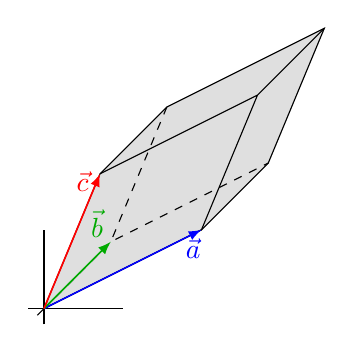
\begin{tikzpicture}[>=latex, scale=1,XYZPersp]	

        % strahlen und koordinatensystem part 1
        \draw[black] (-0.2,0,0)--(1,0,0);
        \draw[black] (0,-0.2,0)--(0,1,0);
        \draw[black] (0,0,-0.2)--(0,0,1);

	\coordinate (a) at (2,0,1);
	\coordinate (b) at (0,2,0);
	\coordinate (c) at (0.5,0.5,1.5);
	\coordinate (aa) at (-2,0,-1);
	\coordinate (bb) at (0,-2,0);
	\coordinate (cc) at (-0.5,-0.5,-1.5);

        \draw[lightgray,fill,opacity=0.5] (0,0,0)--++(a)--++(b)--++(c)--++(aa)--++(bb)--++(cc);
        \draw[black] (0,0,0)--++(a)--++(b)--++(c)--++(aa)--++(bb)--++(cc);
        \draw[black] (0,0,0)--++(a)--++(c)--++(b)--++(bb)--++(aa);
        \draw[black,dashed] (0,0,0)--++(b)--++(a);
        \draw[black,dashed] (0,0,0)--++(b)--++(c);

        \draw[->,blue,semithick] (0,0,0)--(a)node[below=-0.5pt,xshift=-3pt]{ $\vec a$};
        \draw[->,greenT,semithick] (0,0,0)--(b)node[above=-2pt,xshift=-5pt]{ $\vec b$};
        \draw[->,red,semithick] (0,0,0)--(c)node[left=0.5pt,yshift=-3pt]{ $\vec c$};
\end{tikzpicture}
\end{minipage}

\begin{hinweis}
\gaussurl{gausscalc:20000047}
\end{hinweis}

\thema{Determinante}

\begin{loesung}
Das Volumen des Parallelepiped entspricht der Determinante der Matrix 
\[
 A = \begin{pmatrix} 2 & 0 & 1/2\\ 0 & 2 & 1/2\\ 1 & 0 & 3/2\end{pmatrix},
\]
welche sich aus den drei gegebenen Vektoren $\vec a$, $\vec b$ und $\vec c$ zusammensetzt.
Wir berechnen die Determinante von $A$ mit dem Entwicklungssatz und entwickeln nach der zweiten Spalte:
\[
  \det(A) = \left|\,\begin{matrix} 2 & 0 & 1/2\\ 0 & 2 & 1/2\\ 1 & 0 & 3/2\end{matrix}\,\right| 
  = 2\cdot \left|\,\begin{matrix} 2 & 1/2\\ 1 & 3/2\end{matrix}\,\right| 
  = 2 \cdot(2\cdot \dfrac{3}{2}-\dfrac{1}{2}\cdot 1) 
  = 5.
\]
Das Volumen des Parallelepipeds ist somit 5. Das $\det(A) > 0$ bilden die drei Vektoren ein Rechtssystem.
\end{loesung}




